\subsection{Análisis de Rigidez del Mecanismo}
Para el diseño de una herramienta CNC, la precisión es una de las especificaciones más importantes, debido a que esta determina la calidad de los productos, denotando un modo de falla distintivo para estos mecanismos. Puesto que la falta de precisión es producto de las deformaciones a las que está sometido el mecanismo, un método valido para analizar este factor en un mecanismo es el análisis de rigidez del sistema. Más específicamente, el método de elementos finitos, representando la rigidez del mecanismo por medio de matrices de rigidez; las cuales tienen en cuenta comportamientos elásticos y lineales dentro del sistema.

El elemento utilizado para la representación de los cuerpos es el Elemento de Marco Espacial (en inglés, Space Frame Element), por lo que es un elemento finito tridimensional con 12 grados de libertad. Esto es producto de sus dos nodos, los cuales poseen los 3 grados de libertad translaciones y rotacionales cada uno. Aparte de esto, el elemento de marco espacial conserva las siguientes propiedades constantes: Densidad $\rho$, Modulo de Elasticidad $E$, Modulo de Cortante Elástico $G$, Área transversal $A$, Momentos de Inercia de área $I_{y}$ y $I_{z}$, Momento Polar de Inercia $G$ y la longitud $L$.

\begin{figure}[hb!]
    \centering
    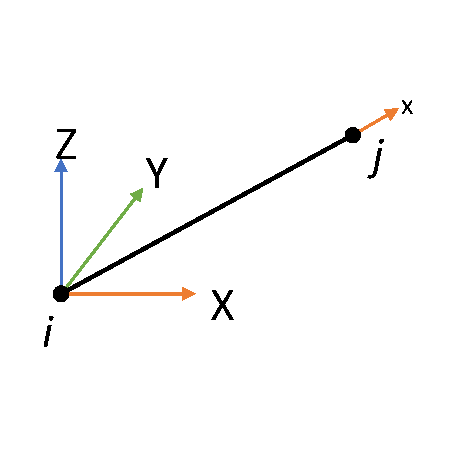
\includegraphics[width=0.30\textwidth]{Cap4_DisenoBasico/Figura/AnalisisRigidez/SPE.pdf}
    \caption{Elemento de Marco Espacial}
    \label{fig:SPE}
\end{figure}

La matriz de rigidez para este elemento es dada por la siguiente matriz:
\begin{equation}
    k = T^{T}k'T
\end{equation}

En donde $T$ es la matriz de rotación del sistema coordenado global al sistema local del elemento, la cual está conformada por $T_{i}$ que es una matriz $3\times3$ de cosenos directores, $T^T$ simboliza la transpuesta de esta matriz, $k$ es la matriz de rigidez del elemento en el sistema global mientras que $k’$ su versión en el sistema local. 

\begin{equation}
    T = \left[ \begin{array}{cccc}
        T_{i} & 0 & 0 & 0 \\
        0 & T_{i} & 0 & 0 \\
        0 & 0 & T_{i} & 0 \\
        0 & 0 & 0 & T_{i}
    \end{array} \right]
\end{equation}

\begin{footnotesize}
\begin{equation}
    k' = \left[\begin{array}{cccccccccccc} \frac{A\, E}{L} & 0 & 0 & 0 & 0 & 0 & -\frac{A\, E}{L} & 0 & 0 & 0 & 0 & 0\\ 0 & \frac{12\, E\, \mathrm{I_z}}{L^3} & 0 & 0 & 0 & \frac{6\, E\, \mathrm{I_z}}{L^2} & 0 & -\frac{12\, E\, \mathrm{I_z}}{L^3} & 0 & 0 & 0 & \frac{6\, E\, \mathrm{I_z}}{L^2}\\ 0 & 0 & \frac{12\, E\, \mathrm{I_y}}{L^3} & 0 & -\frac{6\, E\, \mathrm{I_y}}{L^2} & 0 & 0 & 0 & -\frac{12\, E\, \mathrm{I_y}}{L^3} & 0 & -\frac{6\, E\, \mathrm{I_y}}{L^2} & 0\\ 0 & 0 & 0 & \frac{G\, J}{L} & 0 & 0 & 0 & 0 & 0 & -\frac{G\, J}{L} & 0 & 0\\ 0 & 0 & -\frac{6\, E\, \mathrm{I_y}}{L^2} & 0 & \frac{4\, E\, \mathrm{I_y}}{L} & 0 & 0 & 0 & \frac{6\, E\, \mathrm{I_y}}{L^2} & 0 & \frac{2\, E\, \mathrm{I_y}}{L} & 0\\ 0 & \frac{6\, E\, \mathrm{I_z}}{L^2} & 0 & 0 & 0 & \frac{4\, E\, \mathrm{I_z}}{L} & 0 & -\frac{6\, E\, \mathrm{I_z}}{L^2} & 0 & 0 & 0 & \frac{2\, E\, \mathrm{I_z}}{L}\\ -\frac{A\, E}{L} & 0 & 0 & 0 & 0 & 0 & \frac{A\, E}{L} & 0 & 0 & 0 & 0 & 0\\ 0 & -\frac{12\, E\, \mathrm{I_z}}{L^3} & 0 & 0 & 0 & -\frac{6\, E\, \mathrm{I_z}}{L^2} & 0 & \frac{12\, E\, \mathrm{I_z}}{L^3} & 0 & 0 & 0 & -\frac{6\, E\, \mathrm{I_z}}{L^2}\\ 0 & 0 & -\frac{12\, E\, \mathrm{I_y}}{L^3} & 0 & \frac{6\, E\, \mathrm{I_y}}{L^2} & 0 & 0 & 0 & \frac{12\, E\, \mathrm{I_y}}{L^3} & 0 & \frac{6\, E\, \mathrm{I_y}}{L^2} & 0\\ 0 & 0 & 0 & -\frac{G\, J}{L} & 0 & 0 & 0 & 0 & 0 & \frac{G\, J}{L} & 0 & 0\\ 0 & 0 & -\frac{6\, E\, \mathrm{I_y}}{L^2} & 0 & \frac{2\, E\, \mathrm{I_y}}{L} & 0 & 0 & 0 & \frac{6\, E\, \mathrm{I_y}}{L^2} & 0 & \frac{4\, E\, \mathrm{I_y}}{L} & 0\\ 0 & \frac{6\, E\, \mathrm{I_z}}{L^2} & 0 & 0 & 0 & \frac{2\, E\, \mathrm{I_z}}{L} & 0 & -\frac{6\, E\, \mathrm{I_z}}{L^2} & 0 & 0 & 0 & \frac{4\, E\, \mathrm{I_z}}{L} \end{array}\right]
\end{equation}
\end{footnotesize}

Por consecuencia de la definición del elemento de marco espacial, una estructura con $n$ nodos, la matriz de rigidez de la estructura, $K$, será de $6n\times6n$. Además, para ensamblar la matriz de rigidez global es necesario sumar la submatrices de rigidez de cada elemento en sus respectivos espacios, esto al final genera la siguiente ecuación:

\begin{equation}
    \vec{F} = K \vec{U}
\end{equation}

Donde $\vec{U}$ es un vector que contiene los desplazamientos globales, tanto translaciones como angulares, de todos los nodos y $\vec{F}$ son las fuerzas y momentos globales aplicadas en cada nodo.

Para el modelo del mecanismo en elementos finitos se hicieron dos modificaciones, con el facilitar el modelamiento del mismo (Ver Figura \ref{fig:MecanismoDiscretizado}). La primera modificación fue realizada en la base, que se transformó de una placa triangular con los vértices redondeados a una serie de tubos de rectangular que cumplan la disposición geométrica de la placa forma. La segunda modificación fue eliminar el sistema paralelo de dos ejes sobre el perfil, a solo haber un eje en paralelo con el perfil. Cabe resaltar que el sistema de accionamiento no fue considerado para este análisis.El procedimiento utilizado para el modelo fue obtenido de \cite{kattan2010matlab}.

\begin{figure}[hbt!]
    \centering
    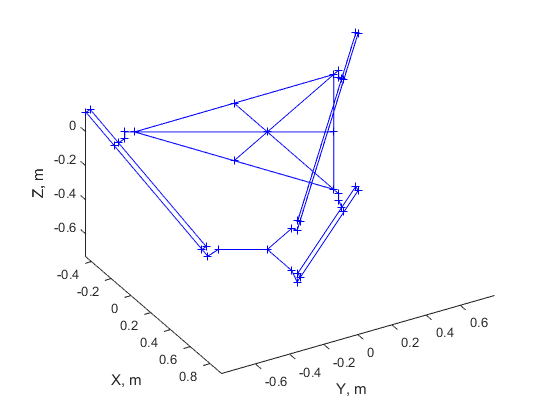
\includegraphics[width=\textwidth]{Cap4_DisenoBasico/Figura/AnalisisRigidez/MecanismoDiscretizado.png}
    \caption{Esquema de la discretización del mecanismo}
    \label{fig:MecanismoDiscretizado}
\end{figure}
\newpage

El modelo manejo dos tipos de material, más específicamente el acero y el aluminio, esto con el objetivo de obtener pesos ligeros en los materiales que no presentan deformaciones significativas y resistencia en aquellos elementos críticos. Los valores utilizados para la simulación son los siguientes:

\begin{longtable}{|c|c|c|c|}
    \hline \rowcolor[gray]{0.85}
    \textbf{Material} & \textbf{Densidad} & \textbf{Modulo de Elasticidad} & \textbf{Modulo de Cortante} \\ \rowcolor[gray]{0.85}
     & $\rho$ [$kg/m^3$] & $E$ [$GPa$] & $G$ [$GPa$] \\ \hline
     Acero & $7850.00$ & $200.00$ & $79.3$ \\ \hline
     Aluminio & $2700.00$ & $69.00$ & $27.00$ \\ \hline
     \caption{Lista de Materiales para el análisis de rigidez}
\end{longtable}

A partir de la discretización del mecanismo (ver Figura \ref{fig:MecanismoDiscretizado}) se establecieron 38 nodos distribuidos en 48 elementos que siguen la siguiente configuración:

\begin{longtable}{|c|c|c|c|c|}
    \hline \rowcolor[gray]{0.85}
    \textbf{Elemento} & \textbf{Material} & \textbf{Perfil Transversal} & \textbf{Componente} & \textbf{Dimensiones} \\ \hline \endhead
     1 : 12 & Acero     & Tuberia Rectangular \Rectpipe & Base          & $B, H, t$ \\ \hline %1
    13 : 15 & Aluminio  & Rectangular $\blacksquare$    & Revoluta AB   & $B, H$ \\ \hline %2
    16 : 18 & Aluminio  & Rectangular $\blacksquare$    & Revoluta AB   & $B, H$ \\ \hline %3
    19 : 21 & Aluminio  & Rectangular $\blacksquare$    & Revoluta BC   & $B, H$ \\ \hline %4
    22 : 24 & Acero     & Circular $\bullet$            & Eje del Brazo & $D$ \\ \hline %5
    25 : 27 & Aluminio  & Rectangular $\blacksquare$    &Soporte del Eje& $B, H$ \\ \hline %6
    28 : 33 & Aluminio  & Viga en T \Tsteel             & Brazo         & $B, H, t$ \\ \hline %7
    34 : 36 & Aluminio  & Rectangular $\blacksquare$    & Revoluta D    & $B, H$ \\ \hline %8
    37 : 39 & Aluminio  & Rectangular $\blacksquare$    & Revoluta DP   & $B, H$ \\ \hline %9
    40 : 42 & Aluminio  & Viga en T \Tsteel             & Brazo         & $B, H, t$ \\ \hline %10
    43 : 45 & Aluminio  & Rectangular $\blacksquare$    &Soporte del Eje& $B, H$ \\ \hline %11
    46 : 48 & Acero     & Rectangular $\blacksquare$    & Eje del Brazo & $B, H$ \\ \hline %12
    \caption{Configuraciones de los elementos}
\end{longtable}

Posterior a esto, las condiciones de frontera utilizadas para resolver este sistema son los nodos $3$, $5$ y $7$ son nodos fijos, es decir, para el análisis no presentan ningún tipo de desplazamiento o empotrados. Además, por las condiciones normales de operación se pueden despreciar los efectos de las aceleraciones dentro del sistema; quedando fuerzas externas al mecanismo, las fuerzas de corte y los pesos de los mismos elementos.